%
% bernoulli.tex
%
% (c) 2024 Prof Dr Andreas Müller
%
\begin{figure}
\centering
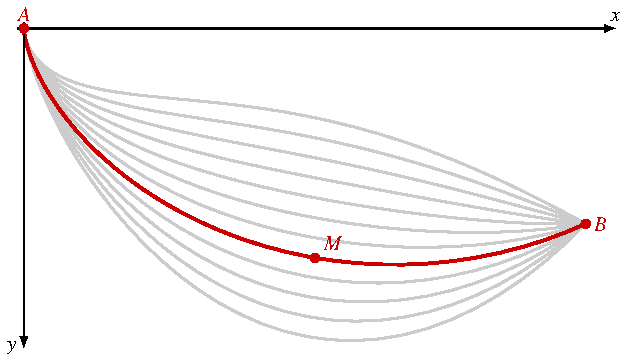
\includegraphics{chapters/020-variation/images/bernoulli.pdf}
\caption{Das Brachistochronenproblem nach Bernoulli.
Auf welchem Weg bewegt sich ein Massepunkt $M$ in der kürzesten
Zeit in einer vertikalen Ebene vom Punkt $A$ zum Punkt $B$ nur unter
dem Einfluss der Schwerkraft?
\label{buch:variation:problem:fig:bernoulli}}
\end{figure}
